\documentclass[12pt]{article}

\usepackage[utf8x]{inputenc}
\usepackage{ucs}
\usepackage{color}
\usepackage{indentfirst}
\usepackage{mathtools}
\usepackage{amsmath}
\usepackage{amsfonts}
\usepackage{amsthm}
\usepackage{amssymb}
\usepackage{enumerate}
\usepackage{listings}
\usepackage{hyperref}
\usepackage{url}
\usepackage{enumitem}
\usepackage[margin=1in]{geometry}
\usepackage[nottoc,numbib]{tocbibind}
\usepackage{combelow}
\usepackage{amsfonts}
\usepackage{multicol}
\usepackage{graphicx}
\usepackage{subcaption}

\setlength{\parskip}{2ex plus 0.5ex minus 0.2ex}
\setcounter{secnumdepth}{2}
\setcounter{section}{-1}
\setlist{nolistsep}

\newcommand{\ddaca}{\Leftrightarrow}
\newcommand{\then}{\Rightarrow}

\newcommand\blfootnote[1]{%
  \begingroup
  \renewcommand\thefootnote{}\footnote{#1}%
  \addtocounter{footnote}{-1}%
  \endgroup
}

\newtheorem{thr}{\bf Teorem\u{a}}[section]
\newtheorem{cor}[thr]{\bf Corolar}
\newtheorem{lema}[thr]{\bf Lem\u{a}}
\newtheorem{prob}[thr]{\bf Problem\u{a}}
\newtheorem{obs}[thr]{\bf Observa\c{t}ie}
\newtheorem{ex}[thr]{\bf Exemplu}
\newtheorem{exs}[thr]{\bf Exemple}
\theoremstyle{definition}
\newtheorem{defi}[thr]{\bf Defini\c{t}ie}
\newtheorem{thr-defi}[thr]{\bf Teorem\u{a}-Defini\c{t}ie}
\newtheorem{nota}[thr]{\bf Nota\cb{t}ie}
\thispagestyle{empty}

\title{Colorizarea pozelor alb-negru}
\date{}
\author{Eric Petru Stavarache}

\begin{document}

\maketitle

\tableofcontents


\begin{abstract}
    Aceasta lucrare trateaza colorizarea pozelor folosind retele adversariale, in particular arhitectura CycleGAN.

    Voi compara rezultatele cu abordarile traditionale.
\end{abstract}

\section{Introducere}

Colorizarea pozelor alb-negru este o sarcina dificila pentru metodele traditionale de invatare.

Una dintre cele mai mari contributii la aceasta dificultate este faptul ca retele traditionale sunt specializate pe minimizarea unei pierderi de tipul $log-loss$ sau $L2$.
Considerand spatiul 3-dimensional al culorilor pixelilor RGB: $\{0, 1, ..., 255 \}^{3}$. Punctele care minimizeaza suma distantelor $L2$ tind sa fie distribuite in jurul culorii gri.
Din aceasta cauza, pozele generate tind sa fie preponderent gri si lipsite de viata.

\section{Munca Anterioara}

Abordarea clasica de colorizare a pozelor este bazata pe retele convolutionale, iar rezultatele din 2016 ale lui Richard Zhang et al sunt impresionante [1][2].
Pentru a rezolva problema distributiei culorilor, ei modifica functia de pierdere pentru a penaliza culorile care nu apar frecvent in poze.
i.e., desi culoarea gri minimizeaza $L2-loss$, nu este intalnita foarte des in pozele adevarate, deci nu va mai fi culoare dominanta in pozele colorizate.


\section{Preliminarii}

\subsection{Notiuni utilizate}

\begin{subsubsection}{Retele generative adversariale}
\begin{defi}
Retelele generative adversariale (eng. Generatv Adversarial Network) au fost inventate de catre Ian Goodfellow in 2014.
Acestea sunt cea mai noua metoda de a rezolva problema esantionarii dintr-un spatiu al datelor unde abordarile traditionale au un bias catre medie. [5].

Aceste retele sunt compuse din doua parti: reteaua generatoare si reteaua discriminatoare.
Reteaua generatoare G incearca sa genereze output din distrubtia $O$, bazandu-se fie pe input din distributia $I$. Vom nota distributia lui G cu $G$.
Reteaua discriminatoare D primeste ca input $i$. D incearca sa distinga daca $i$ a provenit din $O$, distributia adevarata a datelor, sau din $G$, distributia pe care o genereaza G.

Pierderea retelei G este data de cat de bine reuseasca sa "pacaleasca" reteaua D, in timp ce pierderea retelei D este cat de bine reuseste sa distinga intre datele adevarate si cele artificiale.

\end{defi}
Ideea centrala a acestui tip de model se bazeaza pe teoria jocurilor: pe domeniul de min-max. G incearca sa maximizeze scorul, in timp ce D inceaca sa minimizeze scorul.

\begin{figure}
  \centering
  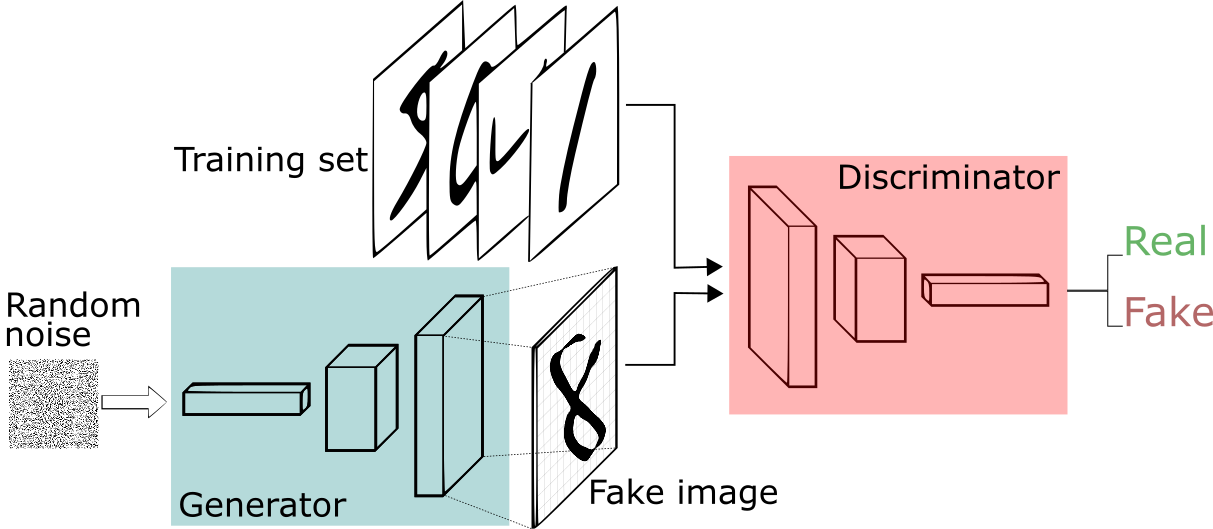
\includegraphics[width=0.7\linewidth]{GAN.png}
  \caption{Retele Adversariale Generative}
  \label{fig:GAN}
\end{figure}

\end{subsubsection}

\subsection{Date de antrenare}

Pentru antrenarea retelei am combinat dataset-urile puse la dispozitie de autorii CycleGAN [6].
Aceste dataset-uri au fost menite pentru a transforma dintr-un domeniu specific in altul (de exemplu de a converti din cai in zebre).
In abordarea mea, am creat reuniunea tuturor pozelor din dataset-uri, deoarece domeniul de poze color include toate celelate poze.
Pentru fiecare poza din reuniune, am generat varianta alb-negru.

\section{Colorizare folosind GAN-uri}

Aceasta lucrare incearca sa trateze problema colorizarii folosind Retele Adversariale Generative - GAN.
Abordarea naiva ar fi formata din cele doua componente clasice: reteaua generatoare si cea discriminatoare.
Reteaua generatoare G primeste o imagine alb-negru si generaza una color.
Reteaua discriminatoare D primeste o imagine color, si incearca sa distinga daca este o imagine naturala, sau daca a fost generata de catre D.

Problema cu aceasta abordare este ca reteaua generatoare descopera ca optim este sa genereze mereu aceeasi poza colorata, fara a tine cont de input. Pentru a rezolva asta, am utilizat abordarea prezentata in \textit{Unpaired Image-to-Image Translation using Cycle-Consistent Adversarial Networks}, sau CycleGAN [3][4].

\subsection{CycleGAN}

CycleGAN este un model care rezolva problema ca output-ul generatorului nu depinde de input.
Ideea centrala este sa avem un generator G1 care ne trece din domeniul $I$ in domeniul $G$ si un generator G2 care ne trece din $G$ in $I$.
Functiile lor de pierdere vor fi corelate de faptul ca vrem ca transformarea inversa sa fie idempotenta.
i.e., daca din alb-negru trecem o poza in color si apoi inapoi in alb-negru, vrem ca cele doua poze alb-negru sa fie cat de similare se poate.

\begin{figure}
  \centering

	\begin{subfigure}{0.4\textwidth}
		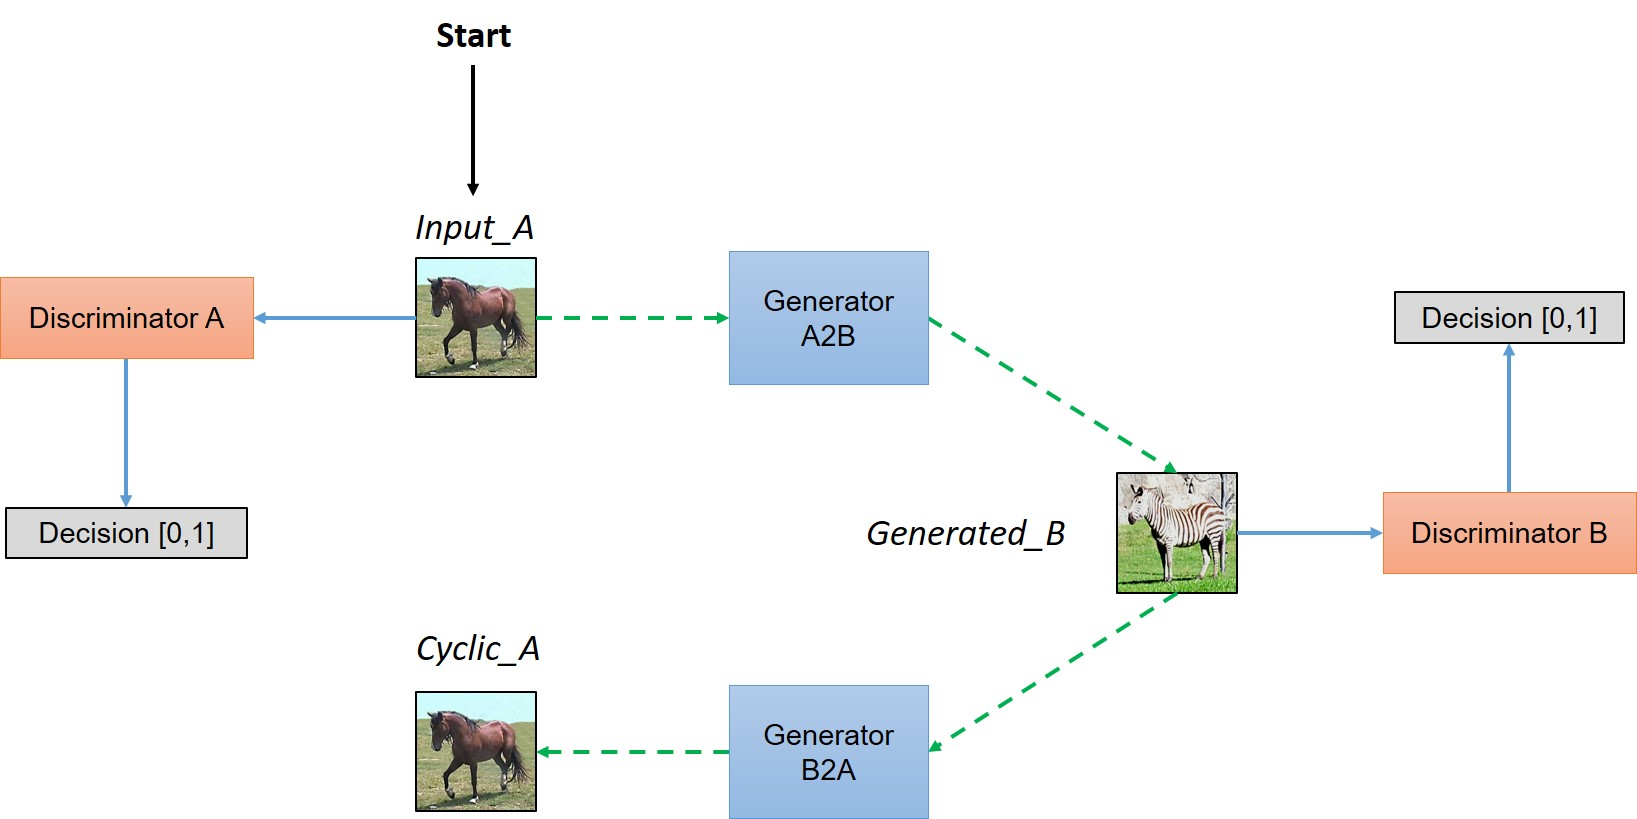
\includegraphics[width=0.5\linewidth]{model.jpg}
		\caption{Ciclul A -> B -> A}
	\end{subfigure}

	\begin{subfigure}{0.4\textwidth}
		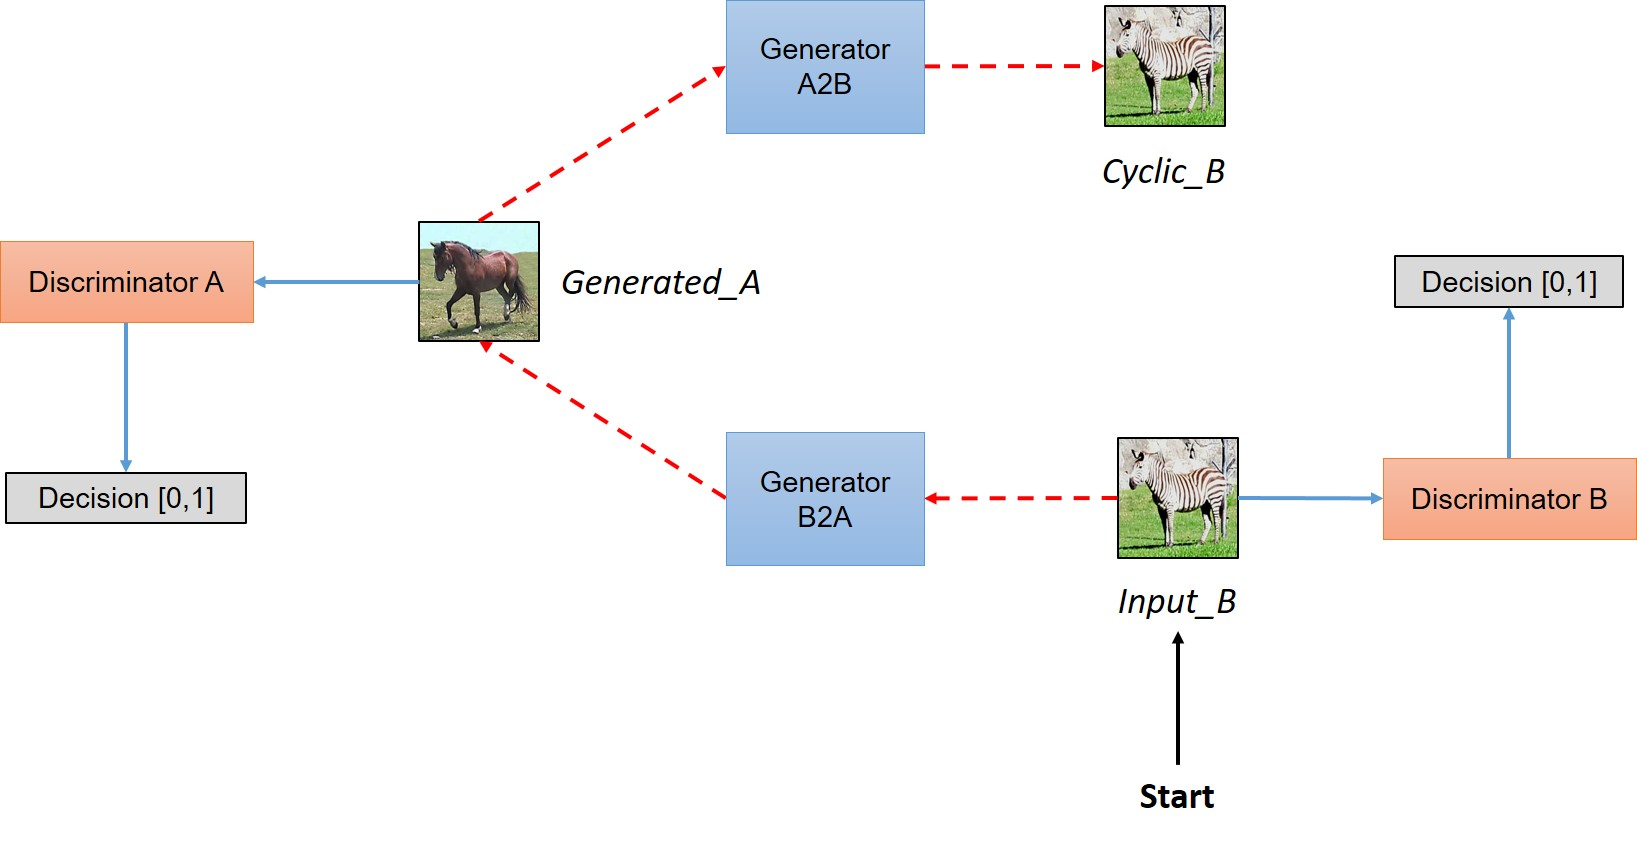
\includegraphics[width=0.5\linewidth]{model1.jpg}
		\caption{Ciclul B -> A -> B}
	\end{subfigure}

  \caption{Modelul de functionare CycleGAN}
  \label{fig:architecture}
\end{figure}


\section{Rezultate si posibile imbunatatiri}

Pozele generate sunt destul de incetosate.
Aceste fapt se genereaza cantitatii mici de date de antrenare folosite, iar o posibila imbunatatire ar fi utilizarea setului de antrenare imagenet

\begin{figure}[h!]
	\centering
	\begin{subfigure}{0.4\textwidth}
		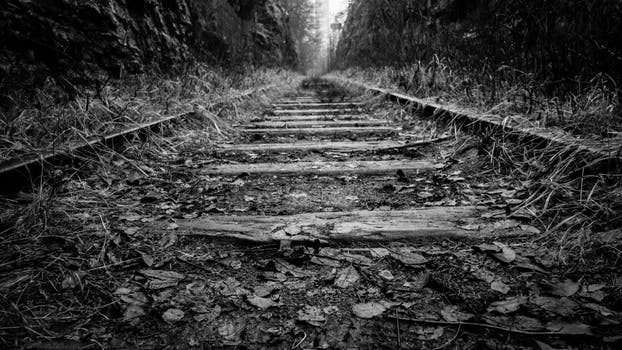
\includegraphics[width=\linewidth]{input_sample.jpg}
		\caption{Poza alb-negru}
	\end{subfigure}
	\vspace{1em}
	\begin{subfigure}{0.4\textwidth}
		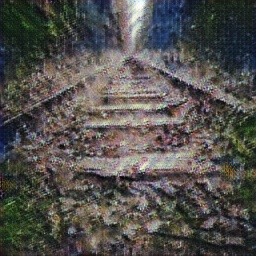
\includegraphics[width=\textwidth]{output_sample.jpg}
		\caption{Poza colorata}
	\end{subfigure}
	\caption{Colorizarea unei poze}
\end{figure}


\section{Bibliografie}

[1] Richard Zang, Phillip Isola, Alexei A. Efros \\ \textit {Colorful Image Colorization}, https://arxiv.org/pdf/1603.08511.pdf, ECCV, 2016. \par
[2] Richard Zang \textit {Colorful Image Colorizaiton}, http://richzhang.github.io/colorization/ \par
[3] Jun-Yan Zhu, Taesung Park, Phillip Isola, Alexei A. Efros, \textit {Unpaired Image-to-Image Translation using Cycle-Consistent Adversarial Networks}, https://arxiv.org/abs/1703.10593 \par
[4] Jun-Yan Zhu, \textit{CycleGAN Project Page}, https://junyanz.github.io/CycleGAN/ \par
[5] Ian J. Goodfellow et al \\ \textit{Generative Adversarial Networks}, https://arxiv.org/abs/1406.2661 \par
[6] Taesung Park, \textit{CycleGAN datasets}, \\ https://people.eecs.berkeley.edu/~taesung\_park/CycleGAN/datasets/ \par

\end{document}
